% !TEX root = ../gnss_interference_resistant_thesis.tex
\documentclass[main.tex]{subfiles}

\begin{document}

\subsection{GNSS signalo krypties nustatymas}\label{sec:gnss_doa_block}

Norint aptikti trigdžių šaltinius (pvz. signalo atspindžius), reikia išmatuoti
signalo priėmimo krypti. Tai galima pasiekti pasinaudojus MUSIC krypties nustatymo
algoritmu (\ref{sec:music} skyrius), tačiau kadangi GPS signalai yra paslėpti triukšmuose
ir visi GPS palydovai transliuoja tame pačiame dažnyje,
tiesiogiai imtuvo duomenims MUSIC taikyti negalime.

Krypties nustatymo įgyvendinimui galime panaudoti GNSS signalo sekimo bloką,
aprašytą \ref{sec:tracking_block} skyriuje. GPS signalo sekimas yra vykodmas
vienoje iš antenų, pvz. $x_0[n]$. Tarpiniai sekimo rezultatai, nešlys ir
nepavėlinta lokali signalo kopija $d_P[k]$, koreliuojami su
kitų antenų signalais, kaip pavaizduota \ref{fig:gnss_sdr_tracking_block_doa}
pav.

\begin{figure}[h]
    \begin{centering}
    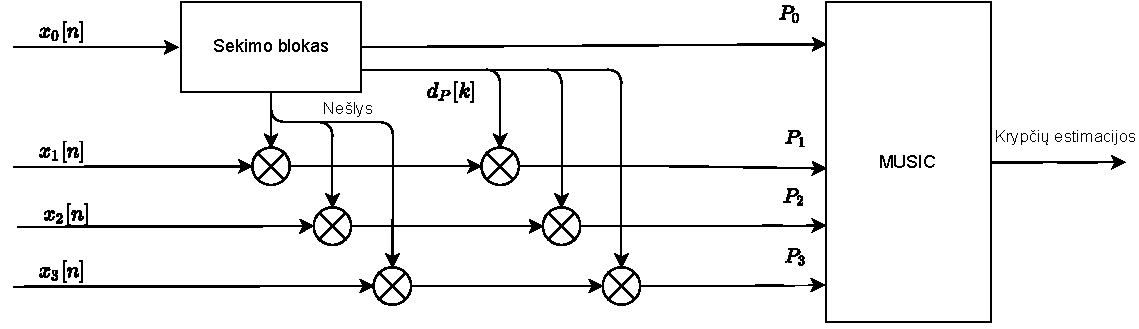
\includegraphics[scale=0.85]{drawings/tracking_diagram_doa}
    \par\end{centering}
    \protect\caption{\label{fig:gnss_sdr_tracking_block_doa}GNSS signalo krypties nustatymo diagrama.}
\end{figure}

Gauti koreliacijos rezultai ($P_n$) yra kompleksiniai skaičiai. šių
rezultatų fazės atspindi priimtų signalų fazes, todėl naudojantis
šiais duomenimis, galime nustatyti signalo atsklidimo kryptį.
Koreliacijos rezultatai yra perduodami MUSIC algoritmui, kuris
įgyvendinimas atliktas naudojantis Python biblioteka "doatools.py" \cite{7738579}.

\ref{fig:gnss_sdr_tracking_block_doa}~pav. blokas yra vykdomas visuose
GNSS imtuvo kanaluose, todėl galime visų matomų palydovų signalų kryptis
nustatyti nepriklausomai. Gavus signalų kryptis ir žinant tikrasias
palydovų padėtis galime pritakyti spindulio formavimo algoritmą
arba pozicijos skaičiavimams nenaudoti palydovų, kurių signalas
yra priimamas netiesiogiai.

\end{document}
